\documentclass[12pt]{article}
\usepackage[pdfborder={0 0 0.5 [3 2]}]{hyperref}%
\usepackage[left=1in,right=1in,top=1in,bottom=1in]{geometry}%
\usepackage[shortalphabetic]{amsrefs}%
\usepackage{amsmath}
\usepackage{enumerate}
% \usepackage{enumitem}
\usepackage{amssymb}                
\usepackage{amsmath}                
\usepackage{amsfonts}
\usepackage{amsthm}
\usepackage{bbm}
\usepackage[table,xcdraw]{xcolor}
\usepackage{tikz}
\usepackage{float}
\usepackage{booktabs}
\usepackage{svg}
\usepackage{mathtools}
\usepackage{cool}
\usepackage{url}
\usepackage{graphicx,epsfig}
\usepackage{makecell}
\usepackage{array}

\def\noi{\noindent}
\def\T{{\mathbb T}}
\def\R{{\mathbb R}}
\def\N{{\mathbb N}}
\def\C{{\mathbb C}}
\def\Z{{\mathbb Z}}
\def\P{{\mathbb P}}
\def\E{{\mathbb E}}
\def\Q{\mathbb{Q}}
\def\ind{{\mathbb I}}

\DeclareMathOperator{\spn}{span}
\DeclareMathOperator{\ran}{range}

\graphicspath{ {periodic/} }

\newtheorem{lemma}{Lemma}
\newtheorem{theorem}{Theorem}
\newtheorem{corollary}{Corollary}
\newtheorem{definition}{Definition}
\newtheorem{assumption}{Assumption}
\newtheorem{hypothesis}{Hypothesis}

\newtheorem{notation}{Notation}

\begin{document}

\section{Rough idea for 2-periodic pulse}

This is a rough sketch only, to see if this will work. Take a standard periodic 2-pulse, $2X_0$ is ``pulse distance'', $2X_1$ is ``period distance''.

\begin{enumerate}

\item Since system is Hamiltonian, we only have one equation we need to solve (SanStrut (3.9) and discussion on p. 2093).

\begin{align}\label{jumpeq}
\langle \Psi(-X_0), Q(X_0) \rangle - \langle \Psi(-X_1), Q(X_1) \rangle + R_0(X_i) &= 0
\end{align}

where $R_0 = \mathcal{O}(e^{-3 \alpha X_m})$, $X_m = \min\{X_i\}$.

\item This is a single equation with two unknowns, so we expect to have a family of solutions paramaterized by one of the unknowns. We can pick either one to be the paramater, but it makes sense to let $X_1$ be the parameter, since the idea is that all periods should be possible. The only possible restriction is that $X_1$ might have to be sufficiently large, but we will deal with that when it comes up. Thus the term $\langle \Psi(-X_1), Q(X_1) \rangle$ will be constant.

\item From Lemma 6.1 in San98, we have an expression for $\langle \Psi(-x), Q(x) \rangle$ for sufficiently large $x$.

\begin{equation}\label{alphabeta}
\langle \Psi(-x), Q(x) \rangle
= s_0 e^{-2 \alpha x} \sin(2 \beta x + \phi) + \mathcal{O}(e^{-(2 \alpha + \gamma) x})
\end{equation}

where $0 < \gamma \leq 1$.

\item Plug \eqref{alphabeta} into \eqref{jumpeq} to get

\begin{align}\label{jumpeq1}
s_0 e^{-2 \alpha X_0} \sin(2 \beta X_0 + \phi) - s_0 e^{-2 \alpha X_1} \sin(2 \beta X_1 + \phi) + \mathcal{O}(e^{-(2 \alpha + \gamma) X_m}) &= 0
\end{align}

The remainder term $R_0$ is incorporated into $\mathcal{O}(e^{-(2 \alpha + \gamma) X_m})$ term, since $R_0$ is equal or higher order.

\item Define the set

\begin{equation}\label{setR}
\mathcal{R} = \left\{ \exp\left(-\frac{\pi \alpha}{\beta}m\right) : m \in \N_0 \right\} \cup \{ 0 \}
\end{equation}

Since $\mathcal{R}$ is closed and bounded, is is compact, thus complete.

\item Define the following things

\begin{align*}
r_m &= e^{-(\pi \alpha /\beta) m} \in \mathcal{R} && m \in \N \\
a_i &= e^{-2\alpha X_i}e^{-\alpha \phi / \beta}\frac{1}{r_m}
\end{align*}

Note that

\begin{align*}
e^{-2 \alpha X_i} &= a_i r_m e^{\alpha \phi / \beta} \\
2 \beta X_i &= -(\beta / \alpha)\log a_i r_m - \phi 
\end{align*}

\item Substitute these into the LHS of \eqref{jumpeq1} to get 

\begin{align}\label{jumpeq2}
s_0 e^{\alpha \phi / \beta } a_0 r_m \sin \left( - \frac{\beta}{\alpha} \log (a_0 r_m) \right) - s_0 e^{\alpha \phi / \beta } a_1 r_m \sin \left( - \frac{\beta}{\alpha} \log (a_1 r_m) \right) + \mathcal{O}(r_m^{1 + \gamma / 2 \alpha}) &= 0 \\
\end{align}

where we have chosen the $X_i$ sufficiently large so that $e^{-2 \alpha X_i} < r_m$ for all $i$. Divide both sides by $r_m$ and the constant $s_0 e^{\alpha \phi / \beta }$ to get

\begin{align}\label{jumpeq3}
a_0 \sin \left( - \frac{\beta}{\alpha} \log (a_0 r_m) \right) - a_1 \sin \left( - \frac{\beta}{\alpha} \log (a_1 r_m) \right) + \mathcal{O}(r_m^{\gamma / 2 \alpha}) &= 0 \\
\end{align}

By the clever choice of $r_m$, as in SanStrut, the $r_m$ term inside the sine terms die, leaving us with

\begin{align}\label{jumpeq4}
a_0 \sin \left( - \frac{\beta}{\alpha} \log a_0 \right) - a_1 \sin \left( - \frac{\beta}{\alpha} \log a_1 \right) + \mathcal{O}(r_m^{\gamma / 2 \alpha}) &= 0 \\
\end{align}

Note that $r_m$ now only occurs in the remainder term, which is what we wanted.

\item We want to use the IFT to solve for $a_0$ in terms of $r_m$, with $a_1$ as a parameter. Thus we want to solve

\begin{align*}
G(a_0, r_m; a_1) = 
a_0 \sin \left( -\frac{\beta}{\alpha} \log a_0 \right) - a_1 \sin \left( - \frac{\beta}{\alpha} \log a_1 \right) + \mathcal{O}(r_m^{\gamma / 2 \alpha}) &= 0
\end{align*}

\item To use the IFT, we need to find values of $a_0$ and $r_m$ so that $G(a_0, r_m; a_1) = 0$. To make things easier, we first take $r = 0$ (which we can do by how we defined $\mathcal{R}$ to get rid of the remainder term, leaving us with

\begin{align*}
G(a_0, 0; a_1) = 
a_0 \sin \left( - \frac{\beta}{\alpha} \log a_0 \right) - a_1 \sin \left( - \frac{\beta}{\alpha} \log a_1 \right)
\end{align*}

With $r_m$ out of the picture, define

\begin{equation}
f(a_0, a_1) = 
a_0 \sin \left( - \frac{\beta}{\alpha} \log a_0 \right) - a_1 \sin \left( - \frac{\beta}{\alpha} \log a_1 \right)
\end{equation}

We are interested in the set of $(a_0, a_1)$ such that this is 0. We note the following.

\begin{enumerate}
	\item $f(a_1, a_0) = -f(a_0, a_1)$, i.e. $f$ is antisymmetric with respect to its two arguments.

	\item $f(a_0, a_0) = 0$. In this case, we have

	\begin{align*}
	G(a_0, r_m; a_0) = \mathcal{O}(r_m^{\gamma / 2 \alpha})
	\end{align*}

	so the lengths $X_i$ (which are the same) drop out of the equation. By the Hamiltonian nature and some handwaving, this has to be satisfied (otherwise there is a jump in the energy). So in this case, we have a 1-periodic wavetrain.

	\item $f(0, 1) = f(1, 0) = 0$. This uses what we know about the limit of the sine term when we approach 0.

   \item We have a family of zeros on the two axes at the points $(0, e^{-n \pi/r})$ and $(e^{-n \pi/r}, 0)$, for $n \in \Z$, where $r = \beta/\alpha$.

\end{enumerate}

We are looking for the zero set of $f(a_0, a_1)$. We know that this zero set contains $a_0 = a_1$, which corresponds to the periodic wavetrain. We also know it contains points on the axes, as described above. By (anti-)symmetry, we only need consider what happens when $a_1 \leq a_0$.\\

Mathematica plotting suggests pitchfork bifurcations take place along the diagonal, and along the branch we will have a periodic double pulse. These bifurcations must take place along the $a_0 = a_1$ line where $f_{a_0}(a_0, a_0) = 0$. (Otherwise we could apply the IFT, and we know that has to give us the line $a_0 = a_1$). Taking this derivative, we get

\begin{align*}
f_{a_0}(a_0, a_0) &= 
\sin \left( - \frac{\beta}{\alpha} \log a_0 \right)
+ a_0 \cos \left( - \frac{\beta}{\alpha} \log a_0 \right)- \frac{\beta}{\alpha} \frac{1}{a_0} \\
&= \sin \left( - \frac{\beta}{\alpha} \log a_0 \right) - \frac{\beta}{\alpha} \cos \left( - \frac{\beta}{\alpha} \log a_0 \right)
\end{align*}

This derivative is 0 when

\begin{align*}
\tan \left( -\frac{\beta}{\alpha} \log a_0 \right) &=  \frac{\beta}{\alpha} \\
-\frac{\beta}{\alpha} \log a_0 &= \arctan \left( \frac{\beta}{\alpha}\right) - n \pi && n \in \Z \\ 
a_0 &= \exp \left( -\frac{\alpha}{\beta} \left( \arctan \left( \frac{\beta}{\alpha}\right) \right) - n \pi \right) && n \in \Z
\end{align*}

We will concern ourselves mainly with the case $n = 0$, so let

\begin{equation}
b^* = \exp \left( -\frac{\alpha}{\beta} \arctan \left( \frac{\beta}{\alpha}\right) \right)
\end{equation}

For $n \in \Z$ let 

\begin{equation}
b^*_n = \exp \left( -\frac{\alpha}{\beta} \left( \arctan \left( \frac{\beta}{\alpha}\right) \right) - n \pi \right) 
= \exp\left(\frac{\alpha}{\beta} n \pi \right) b^*
\end{equation}

Matlab plot suggests that for the pitchfork bifurcation at $b^*_n$, the arms of the pitchfork connect to the points $(0, e^{n \pi/r})$ and $(e^{n \pi/r}, 0)$.

\item Change coordinates so that we can get this (more or less) into the normal form of a pitchfork bifurcation. This is not hard to do, since there is always a zero along the diagonal. Let

\begin{align*}
x &= \frac{1}{2}(a_1 - a_0) \\
y &= \frac{1}{2}(a_1 + a_0)
\end{align*}

Inverting this, we have

\begin{align*}
a_0 &= y - x \\
a_1 &= y + x
\end{align*}

Substituting this into our expression for $f(a_0, a_1)$ yields

\begin{equation}\label{fxy}
f(x, y) = 
(y - x) \sin \left( - \frac{\beta}{\alpha} \log(y - x) \right) - (y + x) \sin \left( - \frac{\beta}{\alpha} \log (y + x) \right)
\end{equation}

It is easy to see from \eqref{fxy} that $f(-x, y) = -f(x, y)$. Thus in terms of the (yet to be proved) pitchfork normal form, the bifurcation parameter is $y$.\\

Using what we did above, we expect that a pitchfork bifurcation will take place at

\begin{equation}\label{pitchpt}
(x_0, y_0) = \left(0, b^* \right) = \left( 0, \exp \left( -\frac{\alpha}{\beta} \arctan \left( \frac{\beta}{\alpha}\right) \right) \right)
\end{equation}

To verify this, we need to check a bunch of derivatives. This is annoying, but not difficult. For the first derivatives, we have

\begin{align*}
f_x(x, y) &= -\sin \left( - \frac{\beta}{\alpha} \log(y - x) \right) - 
\sin \left( - \frac{\beta}{\alpha} \log(y + x) \right) \\
&+\frac{\beta}{\alpha} \cos \left( - \frac{\beta}{\alpha} \log(y - x) \right) + \frac{\beta}{\alpha} \cos \left( - \frac{\beta}{\alpha} \log(y + x) \right) \\
f_y(x, y) &= \sin \left( - \frac{\beta}{\alpha} \log(y - x) \right) - 
\sin \left( - \frac{\beta}{\alpha} \log(y + x) \right) \\
&-\frac{\beta}{\alpha} \cos \left( - \frac{\beta}{\alpha} \log(y - x) \right) + \frac{\beta}{\alpha} \cos \left( - \frac{\beta}{\alpha} \log(y + x) \right)
\end{align*}

Plugging in $(x_0, y_0)$ from \eqref{pitchpt} and noting that 

\begin{align*}
\sin \left( \arctan \left( \frac{\beta}{\alpha}\right) \right) &=
\frac{\beta}{\sqrt{\alpha^2 + \beta^2}} \\
\cos \left( \arctan \left( \frac{\beta}{\alpha}\right) \right) &=
\frac{\alpha}{\sqrt{\alpha^2 + \beta^2}} \\
\frac{\beta}{\alpha} \cos \left( \arctan \left( \frac{\beta}{\alpha}\right) \right) &=
\frac{\beta}{\sqrt{\alpha^2 + \beta^2}} \\
\end{align*}

it is easy to see that both $f_x(x_0, y_0) = 0$ and $f_y(x_0, y_0) = 0$. We now have to check the second derivatives. From Mathematica, we have

\begin{align*}
f_{xx}(x, y) &= -(y-x) \left(-\frac{\beta^2 \sin \left(\frac{\beta \log (y-x)}{\alpha}\right)}{\alpha^2 (y-x)^2}-\frac{\beta
   \cos \left(\frac{\beta \log (y-x)}{\alpha}\right)}{\alpha (y-x)^2}\right)\\
   &+(x+y) \left(-\frac{\beta^2
   \sin \left(\frac{\beta \log (x+y)}{\alpha}\right)}{\alpha^2 (x+y)^2}-\frac{\beta \cos \left(\frac{\beta
   \log (x+y)}{\alpha}\right)}{\alpha (x+y)^2}\right)\\
   &-\frac{2 \beta \cos \left(\frac{\beta \log
   (y-x)}{\alpha}\right)}{\alpha (y-x)}+\frac{2 \beta \cos \left(\frac{\beta \log (x+y)}{\alpha}\right)}{\alpha
   (x+y)}
\end{align*}

Mathematica tells us that $f_{xx}(x_0, y_0) = 0$. It also tells us that $f_{yy}(x_0, y_0) = 0$, although we don't need that for the pitchfork. The mixed derivative $f_{xy}$ is (again from Mathematica)

\begin{align*}
f_{xy}(x, y) &= -\frac{\beta^2 \sin \left(\frac{\beta \log (y-x)}{\alpha}\right)}{\alpha^2 (y-x)}-\frac{\beta^2 \sin
   \left(\frac{\beta \log (x+y)}{\alpha}\right)}{\alpha^2 (x+y)}+\frac{\beta \cos \left(\frac{\beta \log
   (y-x)}{\alpha}\right)}{\alpha (y-x)}+\frac{\beta \cos \left(\frac{\beta \log (x+y)}{\alpha}\right)}{\alpha (x+y)}
\end{align*}

Evaluating this at $(x_0, y_0)$ gives us

\begin{align*}
f_{xy}(x_0, y_0) &= \frac{2\beta}{\alpha\sqrt{\alpha^2 + \beta^2}} \left( \alpha + \frac{\beta^2}{\alpha} \right)\exp\left( \frac{\alpha}{\beta} \arctan \left( \frac{\beta}{\alpha}\right) \right) \\
&= \frac{2 \beta}{\alpha^2}\sqrt{ \alpha^2 + \beta^2 }
\exp\left( \frac{\alpha}{\beta} \arctan \left( \frac{\beta}{\alpha}\right) \right) \\
&= 2 \frac{\beta}{\alpha}\sqrt{ 1 + \left(\frac{\beta}{\alpha}\right)^2 }
\exp\left( \frac{\alpha}{\beta} \arctan \left( \frac{\beta}{\alpha}\right) \right) \\
\end{align*}

Note that this only depends on the ratio $\beta / \alpha$. Since $\alpha, \beta > 0$, $f_{xy}(x_0, y_0) > 0$. Let $k_1 = f_{xy}(x_0, y_0)$. Finally, we check the third derivative with respect to $x$. This is a mess, but from Mathematica we have

\begin{align*}
f_{xxx}(x_0, y_0)
&= -\frac{2 \beta}{\alpha^2}\sqrt{ \alpha^2 + \beta^2 }
\exp\left( \frac{2\alpha}{\beta} \arctan \left( \frac{\beta}{\alpha}\right) \right) \\
&= -2 \frac{\beta}{\alpha}\sqrt{ 1 + \left(\frac{\beta}{\alpha}\right)^2 }
\exp\left( 2 \frac{\alpha}{\beta} \arctan \left( \frac{\beta}{\alpha}\right) \right) < 0\\
\end{align*}

This also only depends on the ratio $\beta / \alpha$. Let $k_2 = -f_{xxx}(x_0, y_0) > 0$. \\

We have verified that a pitchfork bifurcation occurs at $(0, y_0)$. In fact, near the bifurcation point $(0, y_0)$, we have the following Taylor expansion

\begin{align*}
f(x, y) = k_1 x (y - y_0) - \frac{k_2}{6} x^3 + \text{h.o.t.}
\end{align*}

Matlab plot suggests that the two arms of the pitchfork connect to the points $(x,y) = (\pm 1/2, 1/2)$, which correspond to $(a_0, a_1) = (1, 0)$ and $(a_0, a_1) = (0, 1)$. A plot of the arms of the pitchfork from the Taylor expansion together with the zeros of $f(x,y)$ (computed numerically) is given below.

\begin{figure}[H]
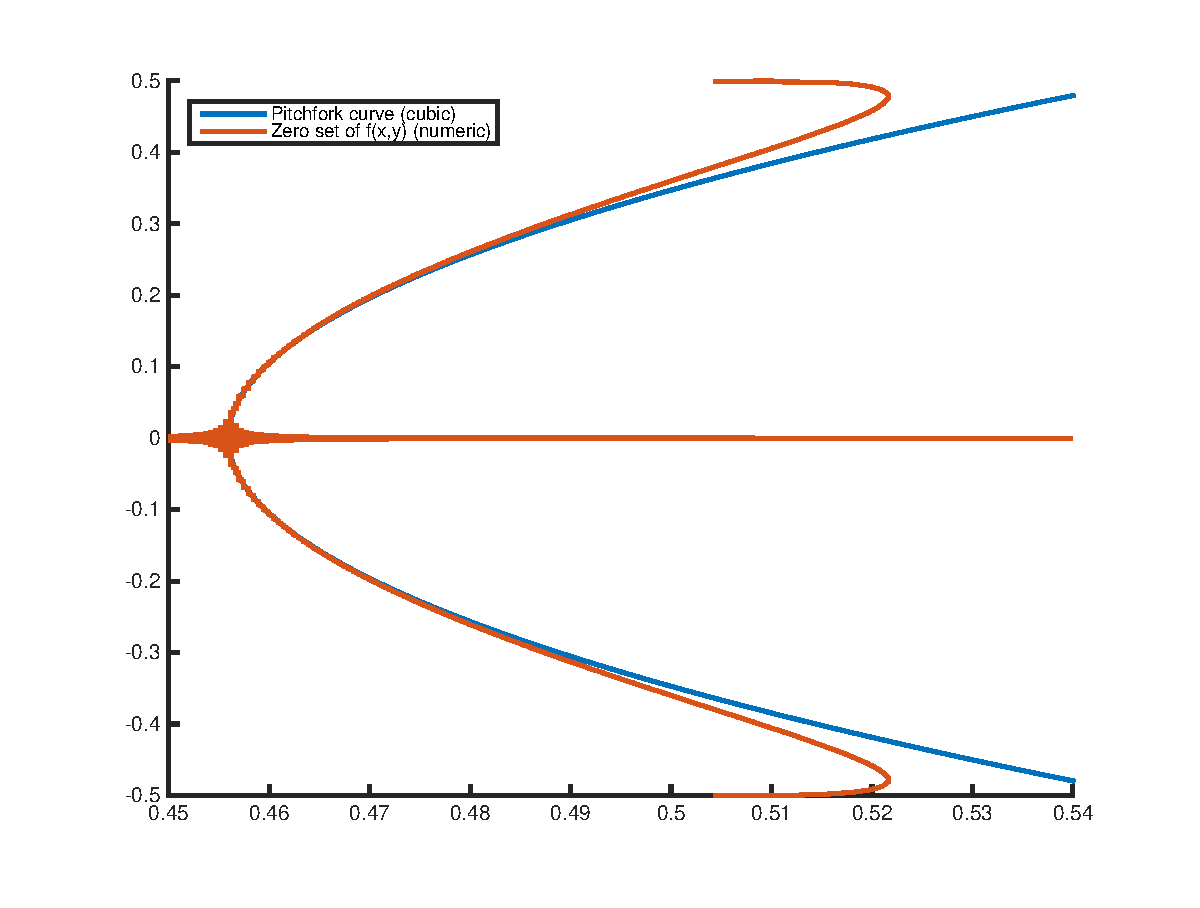
\includegraphics[width=10cm]{pitchfork.eps}
\end{figure}

The pitchfork bifurcation gives us the picture locally near the bifurcation point. We can also look at the ends of the arms at $(x,y) = (\pm 1/2, 1/2)$. Let's look at $(1/2, 1/2)$. Evaluating $f_x(1/2, 1/2)$, we have

\begin{align*}
f_x(1/2, 1/2) &= -\sin \left( - \frac{\beta}{\alpha} \log 1 \right) + \frac{\beta}{\alpha} \cos \left( - \frac{\beta}{\alpha} \log 1 \right)= \frac{\beta}{\alpha} \neq 0
\end{align*}

Since this derivative is not 0, we can use the IFT to solve locally for $y$ in terms of $x$ near $(1/2, 1/2)$. By symmetry, this works near $(-1/2, 1/2)$ as well. \\

Similarly, we can look at the points $(x, y) = (0, b^*_n)$. By the same argument as above, a pitchfork bifurcation occurs at those points as well. 

Thus we have local information in three places. Let's see if we can put them together.\\

\item Consider the following 2-dimensional, first order ODE

\begin{align*}
\dot x &= -f_y(x,y)\\
\dot y &= f_x(x,y)
\end{align*}

where the dot represents differentiation with respect to $t$ (which is just a parameter in this case and has nothing do with with time). By construction, $f(x,y)$ is constant on solutions of this, so we should be able to use it to trace out the curves $f(x,y) = 0$, provided we use the right IC. It is easy to implement this numerically and show that it does what we want.\\

However, this is annoying to deal with in the $(x,y)$ coordinate system. Thus we will switch back to the $(a_0, a_1)$ coordinate system. We also let $r = \beta/ \alpha$ for convenience, since everything only depends on this ratio.

\begin{align}
\dot a_0 &= -f_{a_1}(a_0, a_1) = -[ -\sin(-r \log a_1) 
+ r \cos( -r \log a_1 ) ] \\
\dot a_1 &= f_{a_0}(a_0, a_1) = \sin(-r \log a_0) 
- r \cos( -r \log a_0 )
\end{align}

Here is Matlab output showing this for $r = 5$.

\begin{figure}[H]
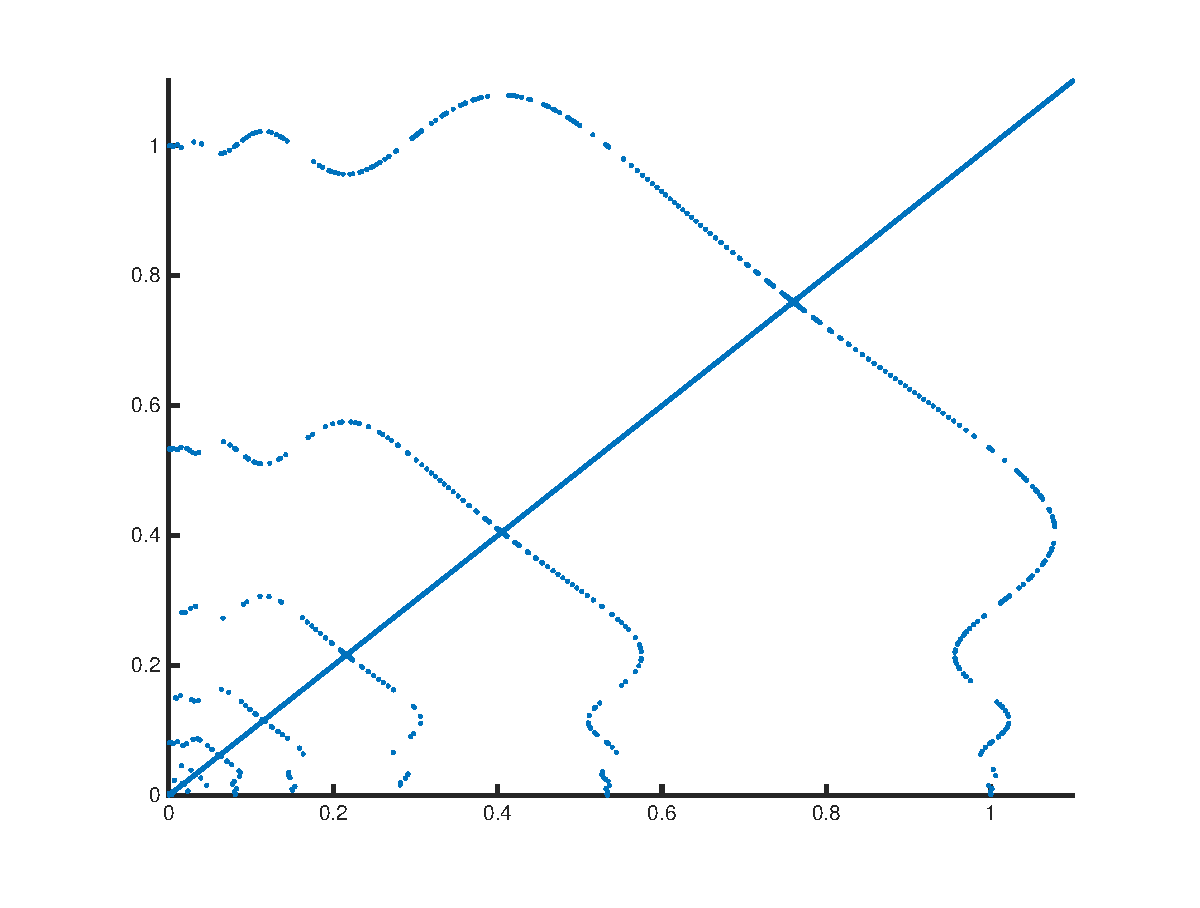
\includegraphics[width=10cm]{zeroset5.eps}
\end{figure}


The advantage here is that each equation only depends on the other variable. Note that $(b^*_n, b^*_n)$ are fixed points of this system (the pitchfork bifurcation points).\\

Also note that 

\begin{align*}
f_{a_0}(a_0, a_1) &= 0 \iff a_0 = b^*_n, n \in \Z \\
f_{a_1}(a_0, a_1) &= 0 \iff a_1 = b^*_n, n \in \Z
\end{align*}

\item It will also be useful to have bounds on the two derivatives of $f$.

\begin{align*}
\frac{d}{d a_0}f_{a_0}(a_0, a_1) &= \frac{1}{a_0} \left(-r \cos(-r \log a_0) - r^2 \sin( -r \log a_0 ) \right) \\
&= -\frac{r}{a_0} \left(\cos(-r \log a_0) + r \sin( -r \log a_0 ) \right)
\end{align*}

Setting this equal to 0, as long as $a_0 \neq 0$, we have

\begin{align*}
\tan(-r \log a_0) &= -1/r \\
-r \log a_0 &= \arctan(-1/r) + n \pi && n \in Z \\
a_0 &= \exp\left( -(1/r) \arctan(-1/r) - n \pi/r \right) && n \in Z \\
\end{align*}

Plugging this into the expression for $f_{a_0}(a_0, a_1)$, we get

\begin{align*}
f_{a_0}(\exp(-(1/r) \arctan(-1/r) - n \pi/r), a_1) &=
\sin(\arctan(-1/r) + n \pi) - r \cos(\arctan(-1/r) + n \pi) \\
&= \pm \left( -\frac{1}{\sqrt{1 + r^2}} - r \frac{r}{\sqrt{1 + r^2}} \right) \\
&= \mp \sqrt{1 + r^2}
\end{align*}

Thus for $a_0 > 0$ and any $a_1$ we have $|f_{a_0}(a_0, a_1)| \leq \sqrt{1 + r^2}$. Similarly, for $a_1 > 0$ and any $a_0$ we have $|f_{a_1}(a_0, a_1)| \leq \sqrt{1 + r^2}$. 

\item Consider the interval $a_0 \in [b^*_n, b^*_{n+1}]$. At the endpoints, $\dot a_1 = f_{a_0}(a_0, a_1) = 0$. There are no other zeros of $f_{a_0}(a_0, a_1)$ between these two points. Consider the point $e^{(2n+1)\pi/(2r) }b^*$ which is between these. Then we have

\begin{align*}
a_1 &= f_{a_0}(e^{(2n+1) \pi / (2r)}b^*, a_1) \\
&= \sin(-r \log e^{(2n+1) \pi / (2r)} b^* ) - r \cos( -r \log e^{(2n+1) \pi / (2r)} b^* ) \\
&= \sin\left(-r \left( \frac{(2n + 1)\pi}{2r} - \frac{1}{r} \arctan r \right) \right) - r \cos\left(-r \left( \frac{(2n + 1)\pi}{2r} - \frac{1}{r} \arctan r \right) \right) \\
&= \sin\left(\arctan r - \frac{\pi}{2} - n \pi \right) - r \cos\left(\arctan r - \frac{\pi}{2} - n \pi \right) \\
&= -\cos\left(\arctan r \right) - r \sin\left(\arctan r\right) \\
&= -(-1)^n \left( \frac{1}{\sqrt{1+r^2}} + r \frac{r}{\sqrt{1+r^2}}  \right) \\
&= (-1)^{n+1}\sqrt{1 + r^2} \neq 0
\end{align*}

Since $\dot a_1 = f_{a_0}(a_0, a_1)$ is continuous on $[b^*_n, b^*_{n+1}]$, is zero only at the endpoints, and is either negative ($n$ even) or positive ($n$ odd) at a point in between, we conclude that on the open interval $(b^*_n, b^*_{n+1})$, $\dot a_1 < 0$ for $n$ even and $\dot a_1 > 0$ for $n$ odd.\\

\item What we would like is a trapping region for solutions which start near the pitchfork bifurcation point. It turns out we can do this, but not in the usual way of showing derivatives point into the region.\\

Consider the bifurcation point $(a_0,a_1) = (b^*_n, b^*_n)$ for any $n \in \Z$. Consider the box with corners $(b^*_n, b^*_n)$, $(b^*_{n+1}, b^*_n)$, $(b^*_n, 0)$, and $(b^*_{n+1}, 0)$. The upper left corner is the pitchfork bifurcation point, and from the normal form we know that the lower branch of the pitchfork goes down and right, so the lower branch enters the box. Within the box, all solutions move down (for $n$ even) or up (for $n$ odd), as we showed above. If a solution hits the bottom edge of the box, it will stop since the RHS of the ODE is singular there. We need to show that the solution cannot exit the sides.\\

We use an energy argument to do this. Take an initial condition $(a_0^*, a_1^*)$ which is on the lower branch of the pitchfork (and thus inside the box). We can do this since we know what happens locally near the pitchfork point. Since the entire pitchfork is contained in the level set $f(a_0, a_1) = 0$, $f(a_0^*, a_1^*) = 0$. Since $f(a_0, a_1)$ is constant along solutions of our ODE and since trajectories cannot cross, it suffices to show that the energy $f(a_0, a_1)$ is nonzero along the sides of the box (except at the corners).\\

Consider the line segment joining $(b^*_n, 0)$ to $(b^*_n, b^*_n)$. Along that line segment we have 

\begin{align*}
f(b^*_n, a_1) &= b^*_n \sin(-r \log b^*_n) - a_1 \sin(-r \log a_1) && a_1 \in (0, b^*_n)\\
\end{align*}

Let $g(x) = x \sin(-r \log x)$. Let $y = -r \log x$, so that $x = e^{-y/r}$. In particular, if $x = b^*_n$, then $y = -r \log b^*_n = \arctan r + n \pi$. Making this substitution, we have $g(y) = e^{-y/r} \sin y$. With this change of variables, it suffices to show that

\begin{align*}
g(\arctan r + n \pi) - g(y) &\neq 0 && y \in (\arctan r + n \pi, \infty) 
\end{align*}

Taking the derivative of $g$ with respect to $y$, we have

\begin{align*}
g'(y) &= e^{-y/r}\left( \cos y - \frac{1}{r} \sin y \right)
\end{align*}

In particular, $g'(\arctan r + n \pi) = 0$, so $\arctan r + n \pi$ is (most likely) either a local min or a local max. (We could have gotten this from the derivatives we computed above and the change of variables). The second derivative is

\begin{align*}
g''(y) &= \frac{e^{-y/r}}{r^2} \left( \sin y - 2 r \cos y - r^2 \sin y \right)
\end{align*}

At $y = \arctan r + n \pi$, this is

\begin{align*}
g''(y) &= (-1)^n e^{-n \pi /r} \frac{e^{-(1/r)\arctan r}}{r^2 \sqrt{1+r^2}} \left( r - 2r - r^3 \right) \\
&= (-1)^{n+1} e^{-n \pi /r} \frac{e^{-(1/r)\arctan r}}{r^2 \sqrt{1+r^2}} r \left( 1 + r^2 \right) \\
&= (-1)^{n+1} e^{-n \pi /r} e^{-(1/r)\arctan r} \frac{ \sqrt{1 + r^2}}{r} \\
&= (-1)^{n+1} p(r)
\end{align*}

where $p(r) > 0$. Thus $\arctan r + n \pi$ is a local max for $n$ even and a local min for $n$ odd. For $n$ even, since $\arctan r + n \pi$ is a local max of $g(y) = e^{-y/r} \sin y$, and we know what that function looks like, $g(y) < g(\arctan r + n \pi)$ whenever $y > \arctan r + n \pi$, thus $g(\arctan r + n \pi) - g(y) > 0$ for $y \in (\arctan r + n \pi, \infty)$. Similarly, if $n$ is odd, $g(y) > g(\arctan r + n \pi)$ whenever $y > \arctan r + n \pi$, thus $g(\arctan r + n \pi) - g(y) < 0$ for $y \in (\arctan r + n \pi, \infty)$. In either case, $g(\arctan r + n \pi) - g(y) \neq 0$ for all $ y \in (\arctan r + n \pi, \infty)$.

\item The solution starting at $(a_0^*, a_1^*)$ evolves along the zero level set of the energy $F$. For $n$ even, we will evolve in forward time, and for $n$ odd, we will evolve in backward time (alternatively, we can replace $F$ with $-F$ for $n$ odd). Solutions will then start in the box, always move down, and are trapped by the sides of the box, since the sides of the box have nonzero energy and trajectories cannot cross. Solutions must terminate at $(e^{n \pi/r}, 0)$. Thus the picture looks (qualitatively) like the Matlab plot.

\item We have fully characterized the level sets $F(a_0, a_1) = 0$. Now we need to show that this bifurcation picture persists for small $r_m$, i.e. the level sets of $G(a_0, r_m; a_1)$ look (qualitatively) like this. Basically we have to show that with a small $r_m$ we still meet the criteria for a pitchfork bifurcation.\\

The first thing we need to show is that we have the same symmetries if the remainder is small and nonzero. We know that $F(a_0, a_1) = -F(a_1, a_0)$. We need to show that $F(a_0, r_m; a_1) = -G(a_1, r_m, a_1)$, at least for sufficiently small $r_m$. Recall that $a_0$ and $a_1$ are functions of the lengths $X_0$ and $X_1$ which we obtain from Lin's method. Suppose we have constructed a solution using Lin's method for lengths $X_0$ and $X_1$. Thus, we have found lengths $X_0, X_1$ which solve

\begin{align}
(U_i^\pm)' - F(U_i^\pm) &= 0 \\
U_0^+(X_0) - U_{1}^-(-X_1) &= 0 \\
U_1^+(X_1) - U_{0}^-(-X_0) &= 0 \\
U_i^+(0) - U_i^-(0) &= 0
\end{align}

\item Eventually, deal with ``duplicate'' solutions, i.e. some combinations of $(a_0, r_m; a_1)$ should give the same solution, as in SanStrut. This will restrict our choice of $a_0$, i.e. tell us which branch of the bifurcation diagram we can use (similar to the restriction in SanStrut that one of the $a_i = 1$.)

\item We now want to use the IFT. So from our bifurcation diagram, we have found a pair $(a_0, a_1)$ such that $F(a_0, a_1) = G(a_0, 0; a_1)= 0$. We want to use the IFT to solve for $a_0$ in terms of $r_m$. The ``periodic parameter'' $a_1$ will remain unchanged.\\

To use the IFT, we need to check the derivative of $G$ with respect to $a_0$ at $(a_0, 0; a_1)$. From above, SanStrut, and the longer writeup, this is

\begin{align*}
\frac{\partial}{\partial a_0} G(a_0, 0; a_1) &=
\frac{\partial}{\partial a_0} a_0 \sin \left( -r \log a_0 \right) \\
&= \sin \left( -r \log a_0 \right) + a_0 \cos \left( -r \log a_0 \right)
\end{align*}

since the derivative of the remainder term with respect to any of the $a_i$ is 0 at $r_m = 0$. Unlike in SanStrut, we cannot compute this exactly. But we showed it is nonzero as long as $a_0 \neq b^*_n$ for any $n$, i.e. as long as we are not at a pitchfork bifurcation point. And if we are at a pitchfork bifurcation point, we don't even need to do this since we have a periodic wavetrain in that case. Thus we can use the IFT. In other words, for sufficiently small $r_m$, there is a function $a_0(r_m)$ with $a_0(0) = a_0$ such that $G(a_0(r_m), r_m; a_1) = 0$.

\item Let $r_0 > 0$ be sufficiently small so that the previous part works. Then chose any $m$ such that $r_m < r_0$. Then we have

\begin{align*}
G(a_0(r_m; a_1), r_m; a_1) = \tilde{G}(a_0(r_m; a_1), r_m; a_1) = 0
\end{align*}

\item What about multipulses. Suppose we are trying to construct an $n$-pulse. In the Hamiltonian case, we need to solve a system of $n - 1$ equations. For $i = 0, \dots, n-2$ we have

\begin{align*}
G_i(a_i, a_{i-1}, r_m) = 
a_i \sin \left( -r \log a_i \right) - a_{i-1} \sin \left( -r \log a_{i-1} \right) + \mathcal{O}(r_m^{\gamma / 2 \alpha}) &= 0 \\
\end{align*}

where as in the double pulse, $a_{n-1}$ will be the periodic parameter. Right now, it only appears in the first equation. Ideally, since $a_{n-1}$ is our parameter, we would each of our equations to involve the parameter as well as one of the other $a_i$. Luckily, that is easy to accomplish using easy linear combinations of the $G_i$. For $i = 0, \dots, n-2$, let

\begin{equation}
\tilde{G}_i = \sum_{j = 0}^i G_i
\end{equation}

Then after canceling terms, we have the equivalent system

\begin{align}
\tilde{G}_i(a_i, r_m; a_{n-1}) = 
a_i \sin \left( -r \log a_i \right) - a_{n-1} \sin \left( -r \log a_{n-1} \right) + \mathcal{O}(r_m^{\gamma / 2 \alpha}) &= 0 \\
\end{align}

\end{enumerate}

\end{document}